\documentclass[11pt,a4paper]{article}
\usepackage[utf8]{inputenc}
\usepackage{tikz}
\usetikzlibrary{decorations.pathreplacing}
\usepackage{microtype}
\usepackage{amsmath}
\usepackage{amsfonts}
\usepackage{amssymb}
\usepackage{xargs}
\usepackage[parfill]{parskip}
\usepackage[margin=1.3in]{geometry}
\usepackage{tabularx}
\usepackage{float}
\usepackage{amsthm}

%\usepackage{ccfonts}
%\usepackage[adobe-utopia]{mathdesign}
%\usepackage{eucal}
%\usepackage{arev}
%\usepackage[T1]{fontenc}
%\usepackage{fontspec}
%\setmainfont{Asana-Math}
%\usepackage[adobe-utopia]{mathdesign}
\usepackage{libertinus}
\usepackage{fdsymbol}
\usepackage[T1]{fontenc}


\usepackage[ruled,vlined,linesnumbered,noend]{algorithm2e}
\usepackage{setspace}

%\def\arraystretch{1.2}

\newcommand{\Qc}{\mathcal{Q}}
\newcommand{\Sc}{\mathcal{S}}
\newcommand{\E}{\mathbb{E}}
\newcommand{\Act}{\mathrm{Act}}
\newcommand{\Ac}{\mathcal{A}}
\newcommand{\dt}{\matrm{\ d}}
\newcommand{\KL}{\mathrm{KL}}
\newcommand{\Af}{\mathbf{A}}
\newcommand{\bfat}{\mathbf{b}}
\newcommand{\xf}{\mathbf{x}}
\newcommand{\af}{\mathbf{a}}
\newcommand{\yf}{\mathbf{y}}
\newcommand{\Df}{\mathbf{D}}
\newcommand{\cf}{\mathbf{c}}
\newcommand{\ef}{\mathbf{e}}
\newcommand{\gf}{\mathbf{g}}
\newcommand{\df}{\mathbf{d}}
\newcommand{\Lc}{\mathcal{L}}
\newcommand{\Uc}{\mathcal{U}}
\newcommand{\Be}{\mathrm{Be}}
\newcommand{\Mult}{\mathrm{Mult}}
\newcommand{\Nc}{\mathcal{N}}
\newcommand{\Fc}{\mathcal{F}}
\newcommand{\R}{\mathbb{R}}
\newcommand{\N}{\mathbb{N}}
\newcommand{\Cov}{\mathrm{Cov}}
\newcommand{\Var}{\mathrm{Var}}
\newcommand{\dom}{\mathrm{dom}}
\newcommand{\st}{\text{subject to}}

\DeclareMathOperator*{\argmax}{\arg\max}
\DeclareMathOperator*{\argmin}{\arg\min}
\newcommand{\pdata}{p_\mathrm{data}}
\newcommand{\pmodel}{p_\mathrm{model}}
\numberwithin{equation}{section}


\newcommand{\idx}{\varphi}
\newcommand{\varidx}{\psi}
\newcommand{\move}[3]{#1_{#2\rightarrow #3}}
\newcommand{\image}{\mathrm{image}}
\newcommand{\minimize}{\text{minimize}}
\renewcommand{\iff}{\quad\text{iff}\quad}

% \newtheoremrep{theorem}{Theorem}[section]
% \newtheoremrep{corollary}{Corollary}[theorem]
% \newtheoremrep{lemma}[theorem]{Lemma}
\newtheorem{definition}{Definition}[section]

% \usepackage{apxproof}
\newtheorem{theorem}{Theorem}[section]
\newtheorem{corollary}{Corollary}[theorem]
\newtheorem{lemma}[theorem]{Lemma}
\newtheorem{theoremrep}{Theorem}[section]
\newtheorem{corollaryrep}{Corollary}[theorem]
\newtheorem{lemmarep}[theorem]{Lemma}
\newcommand{\appendixproof}{proof}

\begin{document}

\tableofcontents
\newpage

% Problem with multicuts: they require a lot of store, since they are bounded by |V|^2.
% Thus, focus on partition-perspective on problem.
% Problem with partitions in set-format: hard to check equalities between partitions set-format and transformations require set-operations that might take a lot of time.
% Therefore: introduce indexings


\section{Notation}
Let $A$ be some set. We will denote the set $\{ \{ a_1, \dots, a_k \} \subseteq A : a_1,\dots,a_k\ \text{distinct}\},$ which contains all $k$-ary subsets of $A$, by $\binom{A}{k}$. For the same set $A$, $P_A$ denotes the set of all partitions of $A$. For a partition $\Pi \in P_A$ and an element $a \in A$, $[a]_\Pi$ denotes the set in $\Pi$ that contains $a$, of which there is exactly one. If $A$ is finite, $\Uc(A)$ denotes the uniform distribution over $A$, i.e. the distribution that assigns every element in $A$ the same probability (namely: $1/|A|$). If we want to indicate that a random variable ${\bf X}$ has probability distribution $\mathcal{Q}$, we will write ${\bf X} \sim \mathcal{Q}$. If $f$ is a function from the domain of a random variable ${\bf X} \sim \mathcal{Q}$ to the real numbers, its expected value is written as $\E_{{\bf X} \sim \mathcal{Q}}\left[f({\bf X})\right]$ and defined as $\E_{{\bf X} \sim \mathcal{Q}} \left[f({\bf X})\right] = \sum_{i=1}^n \mathcal{Q}(x_i) f(x_i)$, if the domain of ${\bf X}$ is finite and given by $\{x_1,\dots,x_n\}$ (we will only consider finite domains).


\section{Introduction}
This work is concerned with the partioning problem with respect to a given finite set $V$, with a cost structure defined over 3-ary subsets of $V$. The considered problem is hard in many respects: one, the amount of possible partitions grows large very fast (with growing $|V|$). Two, even computing the objective function for a given partition is prohibitive, since summing over all $3$-ary subsets takes almost $|V|^3$ steps (and to add to that, not even $|V|^2$ steps are feasible if $|V|$ becomes larger). Thus, we are interested in a way of approximately solving this problem by the use of local search algorithms and some considerations on the objective function. Since the No-Free-Lunch-Theorem (Wolpert et al., \cite{wolpert1995no}) implies that there is no such thing as the ``best'' local search algorithm for arbitrary cost-structures, we want to omit too much focus on specific search algorithms and rather focus on some shared difficulties, e.g. the efficient... 
\begin{itemize}
    \item ...representation of partitions,
    \item ...enumeration of ``neighbours'' for a given partition (possibly in random order)
    \item ...computation (or estimation) of the given cost function and cost-improvements.
\end{itemize}
The problem is given as follows. Let $V = \{ v_1,\dots,v_n \}$ be a finite set, which we will call the set of vertices. Associated with this set are functions $$ c,c': \tbinom{V}{3} \mapsto \R $$ which define a cost-structure on $3$-ary subsets of $V$. For a subset $\{u,v,w\} \in \binom{V}{3}$ and a given partition $\Pi \in P_V$, we define the cost of $\{u,v,w\}$ with respect to $\Pi$ as  
\begin{align*}
    \ell(\{u,v,w\},\Pi) = \begin{cases}
        c(\{u,v,w\}) & \text{if}\ [u]_\Pi \neq [v]_\Pi, [u]_\Pi \neq [w]_\Pi, [w]_\Pi \neq [v]_\Pi \\
        c'(\{u,v,w\}) & \text{if}\ [u]_\Pi = [v]_\Pi = [w]_\Pi \\
        0 & \text{otherwise.}
    \end{cases}
\end{align*}
This can be interpreted as follows: whenever $u,v$ and $w$ are part of pairwise different sets in $\Pi$, the cost of $\{u,v,w\}$ is equal to the costs as defined by $c$. If they are part of the same set, the cost of $\{u,v,w\}$ is equal to the costs as defined by $c'$. Otherwise, if neither of the above is the case, the cost of $\{u,v,w\}$ is just $0$. Based on this definition, we are confronted with problems of the form
\begin{align*}
    \Pi^* = \argmin_{\Pi \in P_V} \sum\nolimits_{\{u,v,w\} \in \binom{V}{3}} \ell(\{u,v,w\},\Pi),
\end{align*}
i.e. we wish to find a partition $\Pi^*$ of $V$ that minimizes some objective function over $3$-ary subsets of $V$. 
\\
In the following section \emph{\nameref{sec:indexings}}, we will discuss an efficient way of representing partitions, e.g. with respect to their space requirements. Afterwards, in section \emph{\nameref{sec:move-operation}}, we consider ways of transforming these representation such that we are able to efficiently generate a neighbourhood (in random order) for each partition. In section \emph{\nameref{sec:objective-function}} we will investigate how the change in the objective function can be computed or estimated, with respect to the neighbourhood of a given partition. The penultimate part \emph{\nameref{sec:algorithms}} contains a theoretic discussion on how the proposed settings influence the runtime of a simple greedy search algorithm, which will be evaluated in section \emph{\nameref{sec:experiments}}. Proofs for Lemmas and Theorems that are shown in this work can be found in the appendix.
\section{Indexings as Proxies for Partitions}\label{sec:indexings}
Since we want to use a local search algorithm that iteratively finds better solutions (partitions in this case), we want to consider on how we want to represent said partitions. One may represent a partition as a set of sets of vertices, which is probably the most straight-forward approach. On the one hand, the required space is linear in $|V|$. But on the other hand, this comes with a few problems: checking if two vertices are part of the same set, and the removal and the addition of a vertex from or to a set all require $|V|$ steps in the worst case (if all vertices have the same set). A last problem is that one has to gurantee feasibility at every step, i.e. that every solution is indeed a partition. A second idea might be to store a partition as a $|V| \times |V|$ boolean matrix, where every row corresponds to a vertex and every column to a set in the partition, and an entry at position $i,j$ would mean ``vertex $i$ is part of set $j$'' if $1$ and ``vertex $i$ is not part of set $j$'' if $0$. This would alleviate some of the above problems, since looking up, removal or addition of vertices to sets would take constant time in the worst case. However, storing a partition would require $|V|^2$ units of space, which might become problematic when $|V|$ is large or when considering multiple partitions at once.

Therefore, we will use the following concept of indexings (which induce equivalence relations on $V$) to solve the above problems, i.e. to simplify and speed up operations on partitions. Every vertex is mapped to a number (index) which indicates the set in the partition we want this vertex to be a part of. If multiple vertices are mapped to the same index, they will be part of the same set in the partition. Since there are at maximum $|V|$ sets in a partition of $V$ (every vertex is assigned its own set, i.e. the indexing is bijective), we restrict to indices between $1$ and $|V|$. Note that every indexing can be stored in space $O(|V|)$.


\begin{figure}[ht]
    \centering
    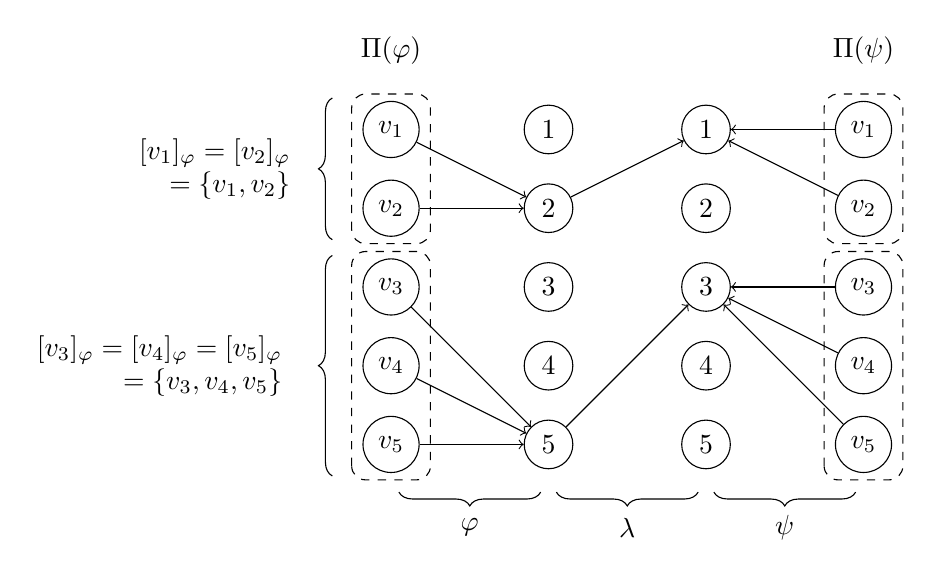
\begin{tikzpicture}
    
    \foreach \s in {1,...,5} {
        \node[draw, circle] (vl\s) at (0,5-\s) {$v_\s$};
        \node[draw, circle] (nl\s) at (2,5-\s) {$\s$};
        \node[draw, circle] (nr\s) at (4,5-\s) {$\s$};
        \node[draw, circle] (vr\s) at (6,5-\s) {$v_\s$};
    }

    \draw[->] (vl1) -- (nl2);
    \draw[->] (vl2) -- (nl2);
    \draw[->] (vl3) -- (nl5);
    \draw[->] (vl4) -- (nl5);
    \draw[->] (vl5) -- (nl5);

    \draw[->] (vr1) -- (nr1);
    \draw[->] (vr2) -- (nr1);
    \draw[->] (vr3) -- (nr3);
    \draw[->] (vr4) -- (nr3);
    \draw[->] (vr5) -- (nr3);

    \draw[->] (nl2) -- (nr1);
    \draw[->] (nl5) -- (nr3);


    \draw [decorate,decoration={brace,amplitude=5pt,mirror,raise=4ex}](0.1,0) -- (1.9,0) node[midway,yshift=-3em]{$\idx$};

    \draw [decorate,decoration={brace,amplitude=5pt,mirror,raise=4ex}](2.1,0) -- (3.9,0) node[midway,yshift=-3em]{$\lambda$};

    \draw [decorate,decoration={brace,amplitude=5pt,mirror,raise=4ex}](4.1,0) -- (5.9,0) node[midway,yshift=-3em]{$\varidx$};

    \node at (0,5) {$\Pi(\idx)$};
    \draw [decorate,decoration={brace,amplitude=5pt,raise=4ex},xshift=-4pt,yshift=0pt,align=right](0,-0.4) -- (0,2.4) node [black,midway,xshift=-2.8cm] {$[v_3]_\idx = [v_4]_\idx = [v_5]_\idx$ \\ $= \{v_3,v_4,v_5\}$};
    \draw [decorate,decoration={brace,amplitude=5pt,raise=4ex},xshift=-4pt,yshift=0pt,align=right](0,2.6) -- (0,4.4) node [black,midway,xshift=-2.1cm] {$[v_1]_\idx = [v_2]_\idx$\\ $= \{v_1,v_2\}$};
    \draw[rounded corners=5pt, dashed] (-0.5,-0.45) rectangle (0.5,2.45);
    \draw[rounded corners=5pt, dashed] (-0.5,3-0.45) rectangle (0.5,3+1.45);

    \node at (6,5) {$\Pi(\varidx)$};
    \draw[rounded corners=5pt, dashed] (6-0.5,-0.45) rectangle (6+0.5,2.45);
    \draw[rounded corners=5pt, dashed] (6-0.5,3-0.45) rectangle (6+0.5,3+1.45);

    \end{tikzpicture}
    \captionsetup{width=.9\linewidth}
    \caption{Illustration of two indexings $\idx,\varidx$ with corresponding partitions and proof of equality through part (b) of Theorem \ref{theorem:equal_indexings}.}\label{fig:indexings}
\end{figure}

\begin{definition}
    Let $V = \{ v_1,v_2,\dots, v_n \}$ be a set of vertices. An indexing of $V$ is a mapping $\idx \in \{ 1,\dots,n \}^V = [n]^V$ that associates every vertex with a number from 1 to $n$. \label{def:indexings}
\end{definition}

\begin{definition}
    Let $\idx$ be an indexing of $V$. The partition induced by $\idx$ is defined as
    \begin{equation}
        \Pi(\idx)= \{ [v]_\idx : v \in V \}, \label{eq:indexing}
    \end{equation}
    where $[v]_\idx = \{ w \in V : \idx(w) = \idx(v) \}$. \label{def:indexing_partition}
\end{definition}

Based on definition \ref{def:indexings} and \ref{def:indexing_partition}, we are able to obtain some immediate results. First, we are able to use indexings as representations for partitions, i.e. for every partition, there is some indexing that yields that very partition (Lemma \ref{lemma:indexing_partition}). And two, we obtain a criterion that makes it possible to check when two vertices share the same set in the partition (Lemma \ref{lemma:indexing_same_set}).  

\begin{samepage}
    \begin{lemmarep}
        $\Pi$ partitions $V$ if and only if there exists an indexing of $V$ that induces $\Pi$.\label{lemma:indexing_partition}
    \end{lemmarep}
\end{samepage}
\begin{proof}
    First, we will show the direction from left to right. Let $\Pi = \{U_1,\dots,U_m\}$, $1\leq m \leq n$, be a partition of $V$. For all vertices $v$ with corresponding set $U_i$ in $\Pi$ (of which there is exactly one), we define $\idx(v) = i$. For a $j \in \{1,\dots,m\}$ we then obtain $\idx^{-1}(j) = U_j$. But then $\Pi(\idx) = \Pi$, i.e. $\Pi$ is induced by $\idx$. 
    \\
    The other direction requires us to prove that every indexing induces a partition of $V$. I.e., for an indexing $\idx$ of $V$ with $\Pi(\idx)=\Pi$, we need to check the following requirements:
    \begin{enumerate}
        \item $\emptyset \not\in \Pi$:\quad This is obvious from \eqref{eq:indexing}, since every element $[v]_\idx \in \Pi$ contains $v$. %https://en.wikipedia.org/wiki/Partition_of_a_set
        \item $\bigcup_{U \in \Pi} U = V$:\quad ``$\subseteq$'' is obvious. For ``$\supseteq$'', take a vertex $v$. Then, $v \in [v]_\idx$ and since $[v]_\idx \in \Pi(\idx)$, we obtain $v \in \bigcup_{U \in \Pi} U$.
        \item if $U_1,U_2 \in \Pi$ and $U_1 \neq U_2$, then $U_1 \cap U_2 = \emptyset$:\quad Take two $U_1, U_2 \in \Pi$ with $U_1 \neq U_2$ such that $U_1 = [w]_\idx$ and $U_2 = [u]_\idx$ for two vertices $w$ and $u$. Assume for a contradiction that $U_1 \cap U_2 \neq \emptyset$, i.e. there exists $v \in U_1 \cap U_2$. But then $v \in [w]_\idx$ and $v \in [u]_\idx$. Thus, $\idx(v) = \idx(w) = \idx(u)$, which cannot be the case, since that would imply $U_1 = U_2$.
    \end{enumerate}
    This completes the proof.
\end{proof}

\begin{samepage}
    \begin{lemmarep}
        Let $\idx$ be an indexing of $V$. For all vertices $v,u$, we have $\idx(v) = \idx(u)$ if and only if $v$ and $u$ are part of the same set in $\Pi(\idx)$. \label{lemma:indexing_same_set}
    \end{lemmarep}
\end{samepage}
\begin{proof}
    For the direction from left to right, take $v,u\in V$ such that $\idx(v)=\idx(u)$. Then $v,u \in [v]_\idx = [u]_\idx \in \Pi(\idx)$, i.e. they are part of the same set. For the other direction, we will show the contraposition. Take $v,u\in V$ such that $\idx(v)\neq \idx(u)$. Clearly, $v \in [v]_\idx$ and $v \not\in [u]_\idx$ as well as $u \in [u]_\idx$ and $u \not\in [v]_\idx$. Therefore $[v]_\idx \neq [u]_\idx$. Since by Lemma \ref{lemma:indexing_partition}, $\Pi(\idx)$ is a partition and $[v]_\idx$ and $[u]_\idx$ are distinct sets in $\Pi(\idx)$, $[v]_\idx$ is the only set that contains $v$ and vice versa for $[u]_\idx$ and $u$. Thus, $v$ and $u$ cannot be part of the same set in $\Pi(\idx)$. 
\end{proof}

Since we want to use indexings in order to define transformations on partitions, we are interested in the question when two indexings are ``equal'', in the sense that they induce the same partition. This is characterized in part by Theorem \ref{theorem:equal_indexings}.

\begin{samepage}
    \begin{theoremrep}
        If $\idx,\varidx$ are two indexings of $V$, then the following statements are equivalent:
        \begin{enumerate}
            \item[(a)] $\Pi(\idx)=\Pi(\varidx)$
            \item[(b)] there is a bijection $\lambda : \image(\idx) \rightarrow \image(\varidx)$\footnote{$\image(\idx)$ means the image of $\idx$, i.e. $\image(\idx)=\{ \idx(v) \}_{v \in V}$.} such that $\lambda(\idx(v)) = \varidx(v)$ \\ for all $v \in V$
            \item[(c)] for all vertices $v,w$, $\idx(w) = \idx(v)$ if and only if $\varidx(w) = \varidx(v)$
        \end{enumerate} \label{theorem:equal_indexings}
    \end{theoremrep}
\end{samepage}
\begin{proof}
    We will start with the direction from (a) to (b). Let $\idx$, $\varidx$ be two indexings of $V$ with $\Pi(\idx) = \Pi(\varidx)$. We define $\lambda : \image(\idx)\rightarrow \image(\varidx)$ as follows. For all $k \in \image(\idx)$, associate a vertex $v$ such that $\idx(v)=k$. Then define $\lambda(k)=\varidx(v)$. It remains to show that $\lambda$ fulfills the requirements in (b):
    \begin{enumerate}
        \item $\lambda$ is bijective:\quad Since every element in $\image(\idx)$ corresponds to a set in $\Pi(\idx)$, and vice versa for $\image(\varidx)$ and $\Pi(\varidx)$, we get $|\image(\idx)|=|\Pi(\idx)|=|\Pi(\varidx)|=|\image(\varidx)|$. Since $\image(\idx)$ and $\image(\varidx)$ are also finite, it suffices to show injectivity of $\lambda$ in order to prove bijectivity. Assume for a contradiction that $\lambda$ is not injective, i.e. there are $v_1,v_2 \in V, \idx(v_1) \neq \idx(v_2)$, such that $\lambda(\idx(v_1))=\lambda(\idx(v_2))=\varidx(v_1)=\varidx(v_2)$. Thus, by application of Lemma \ref{lemma:indexing_same_set}, there must be a set in $\Pi(\varidx)$ that contains $v_1$ and $v_2$, while there is no set in $\Pi(\idx)$ that has both vertices in it. But then $\Pi(\idx)\neq \Pi(\varidx)$. Contradiction.
        \item For all vertices $v$, $\lambda(\idx(v)) = \varidx(v)$: \quad Take an arbitrary vertex $v$ and let $\idx(v) = k \in \image(\idx)$. Let $\bar{v}$ be the vertex that was previously associated with $k$ in the definition of $\lambda$, i.e. the vertex for which $\idx(\bar{v})=k = \idx(v)$ and $\lambda(\idx(\bar{v}))=\varidx(\bar{v})$ holds. Assume for a contradiction that $\varidx(v)\neq \varidx(\bar{v})$. By Lemma \ref{lemma:indexing_same_set}, this yields that there is no set in $\Pi(\varidx)$ that contains both $v$ and $\bar{v}$, while there is one in $\Pi(\idx)$. But then again $\Pi(\idx) \neq \Pi(\varidx)$, i.e. a contradiction. Thus, $\lambda(\idx(v)) = \lambda(\idx(\bar{v})) = \varidx(\bar{v}) = \varidx(v)$. 
    \end{enumerate}
    This concludes this direction. For the direction from (b) to (c), let $\lambda$ be a bijection between the images of two indexings $\idx, \varidx$ of $V$ that fulfills the requirements in (b). Let $w,v$ be two arbitrary vertices; then
    \begin{align*}
        \idx(w) = \idx(v) &\quad\text{iff}\quad \lambda(\idx(w)) = \lambda(\idx(v)) &(*) \\ 
        &\quad\text{iff}\quad \varidx(w) = \varidx(v) &(**)
    \end{align*}
    The first identity $(*)$ works since $\lambda$ is a bijection and the second $(**)$ since $\lambda(\idx(w))=\varidx(w)$ for all vertices $w$.
    The remainder (c) to (a) is relatively trivial: If we assume premise (c), then
    \begin{align*}
        U \in \Pi(\idx) &\quad\text{iff}\quad U = [v]_\idx \text{ for a vertex $v$} \\
        &\quad\text{iff}\quad U = \{ w \in V : \idx(w) = \idx(v) \} \text{ for a vertex $v$} \\
        &\quad\text{iff}\quad U = \{ w \in V : \varidx(w) = \varidx(v) \} \text{ for a vertex $v$} \\ 
        &\quad\text{iff}\quad U = [v]_{\varidx} \text{ for a vertex $v$} \\
        &\quad\text{iff}\quad U \in \Pi(\varidx),
    \end{align*}
    which shows $\Pi(\idx)=\Pi(\varidx)$.
\end{proof}

If the task is to determine whether two induced partitions $\Pi(\idx)$, $\Pi(\varidx)$ for given indexings $\idx,\varidx$ of $V$ are equal, the result of Theorem \ref{theorem:equal_indexings} might be useful: instead of explicitly computing the resulting partitions and checking if both sets are equal, one can simply determine whether a fitting bijection $\lambda$ exists, which is arguably easier. In fact, one can construct $\lambda$ as in the first part of the proof of Theorem \ref{theorem:equal_indexings} and then check whether the result is a bijection or not. Figure \ref{fig:indexings} illustrates two indexings, their partitions and some of the findings of Theorem \ref{theorem:equal_indexings}.


%\bibliography{column_generation}{}
%\bibliographystyle{plain}

\end{document}